\documentclass[11pt]{article}

\usepackage[scale=1]{ccicons}
\usepackage{metalogo}
\usepackage{xcolor,colortbl}
\usepackage{multicol,multirow,booktabs}
\usepackage{graphicx}
\usepackage{bm}
\usepackage{fontawesome5}
\usepackage{xsim}
% Definir un nuevo tipo de ejercicio llamado "Pregunta"
\DeclareExerciseType{pregunta}{
  exercise-env = pregunta,
  solution-env = respuesta,
  exercise-name = Pregunta,
  solution-name = Respuesta,
  exercise-template = simple,
  solution-template = simple,
}

\usepackage[paper=a4paper, headheight=110pt,showframe=false, 
            layoutvoffset=2em,
            bottom=2cm, top=3.5cm, left=2.5cm, right=2.0cm]{geometry}
\usepackage[spanish, es-nodecimaldot]{babel}
\DeclareExerciseTranslations{exercise}{
  Fallback = exercise,
  English = exercise,
  Spanish = ejercicio
}
\usepackage{hyperref}
\usepackage{amsmath}
\usepackage{mismath}
\usepackage{gensymb,amssymb}
\setlength{\parindent}{3em}
\setlength{\parskip}{1em} 
\usepackage[shortlabels]{enumitem}
\usepackage{subcaption}
\usepackage{wrapfig}
\usepackage{siunitx}
%\usepackage{mathspec}
%\usepackage{unicode-math}


% Fonts can be customized here.
\defaultfontfeatures{Mapping=tex-text}
\setmainfont [Ligatures={Common}]{Linux Libertine O}
\setmonofont[Scale=0.9]{Linux Libertine Mono O}
%\usepackage[svgnames]{xcolor} % Gestión de colores
\usepackage{hyperref}
\hypersetup{
  colorlinks=true, linktocpage=true, pdfstartpage=3, pdfstartview=FitV,%
  breaklinks=true, pageanchor=true,%
  pdfpagemode=UseNone, %
  plainpages=false, bookmarksnumbered, bookmarksopen=true, bookmarksopenlevel=1,%
  hypertexnames=true, pdfhighlight=/O,%nesting=true,%frenchlinks,%
  urlcolor=Maroon, linkcolor=RoyalBlue, citecolor=Blue, %pagecolor=RoyalBlue,%
  pdftitle={},%
  pdfauthor={\textcopyright\ C. Manuel Carlevaro},%
  pdfsubject={},%
  pdfkeywords={},%
  pdfcreator={XeLaTeX},%
  pdfproducer={XeLaTeX}%
}

%% Operadores
\DeclareMathOperator{\sen}{sen}
\DeclareMathOperator{\senc}{senc}
\DeclareMathOperator{\sign}{sign}
\newcommand{\T}[1]{\underline{\bm{#1}}}
\DeclareMathOperator{\Tr}{Tr}
%\NewDocumentCommand{\evalat}{sO{\big}mm}{%
  %\IfBooleanTF{#1}
   %{\mleft. #3 \mright|_{#4}}
   %{#3#2|_{#4}}%
%}

\xsimsetup{
solution/print = true
%solution/print = false
}

\title{Introducción a la física}
\author{Manuel Carlevaro}
\date{Universidad de Navarra}


\begin{document}
%\maketitle

\begin{center}
\framebox[1.0\textwidth][c]{
\huge{\textsc{Introducción a la física}} 
}
\end{center} 

\begin{center}
\vspace{1em}
\Large{\textsc{Universidad de Navarra}} 
\end{center}

 \vspace{1em}

\begin{center}
\begin{tabular}{r l}
 \textbf{Tema:} & Cinemática.\\
 \textbf{Profesor:} & Manuel Carlevaro \\
 \textbf{Ayudante:} & Alba Meneses Felipe
\end{tabular}\end{center}

\vspace{2em}

\begin{exercise}
    Un conductor que viaja a rapidez constante de \qty{15}{m/s} pasa por un cruce escolar, cuyo límite de velocidad es de \qty{10}{m/s}. En ese preciso momento, un oficial de policía en su motocicleta, que está parado en el cruce, arranca para perseguir al infractor, con aceleración constante de \qty{3.0}{m/s^2} . Se muestran cuatro posibles gráficas $v_x - t$ para los dos vehículos. ¿Cuál es la gráfica correcta?
\begin{center}
    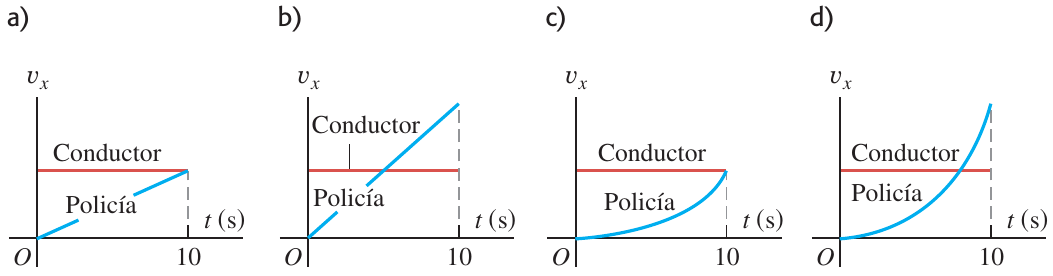
\includegraphics[width=0.9\textwidth]{figs/activ-01.png}
\end{center}
\end{exercise}
\begin{solution}
    La opción correcta es la b).
\end{solution}

\begin{exercise}
La figura muestra una serie de fotografías de alta rapidez (a intervalos de tiempo iguales) de un insecto que vuela en línea recta de izquierda a derecha (en la dirección $+x$). ¿Cuál de las gráficas siguientes es más probable que describa el movimiento del insecto?
\begin{center}
    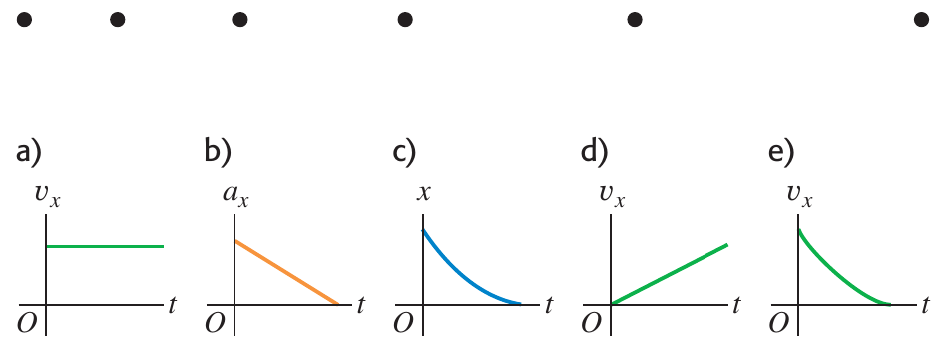
\includegraphics[width=0.9\textwidth]{figs/activ-02.png}
\end{center}
\end{exercise}
\begin{solution}
    La opción correcta es la d).
\end{solution}

\begin{exercise}
Un conductor fue citado en el tribunal por exceso de rapidez. La prueba contra el conductor era que una mujer policía observó al automóvil del conductor junto a un segundo auto, en un momento en que la mujer policía ya había determinado que el segundo auto excedía el límite de rapidez. El conductor alegó que: “el otro auto me estaba rebasando, y yo no iba a exceso de rapidez”. El juez dictaminó contra él porque, según dijo, “si los autos estaban juntos, ambos iban a exceso de rapidez”. Si usted fuera la abogada del conductor, ¿cómo defendería su caso?
\end{exercise}
\begin{solution}
Construir un gráfico de posición como función del tiempo para mostrar que cuando uno
rebasa a otro sus velocidades no son iguales.
\end{solution}

\begin{exercise}
Un automóvil viaja al oeste. ¿Puede tener una velocidad hacia el oeste y simultáneamente una aceleración hacia el este? ¿En qué circunstancias?
\end{exercise}
\begin{solution}
    Si. Cuando está frenando.
\end{solution}

\begin{exercise}
    En un experimento, se sacó a una ave marina de su nido, se le llevó a \qty{5150}{km} de distancia y luego fue liberada. El ave regresó a su nido \num{13.5} días después de haberse soltado. Si el origen es el nido y extendemos el eje $+x$ al punto de liberación, ¿cuál fue la velocidad media del ave en \unit{m/s} en el vuelo de regreso? ¿Y desde que se sacó del nido hasta que regresó?
\end{exercise}
\begin{solution}
    Velocidad media $= \qty{4.42}{m/s}$. Desde que se sacó del nido hasta que regresó la velocidad media es \qty{0}{m/s}.
\end{solution}

\begin{exercise}
Los terremotos producen varios tipos de ondas de choque. Las más conocidas son las ondas P (P por primaria o presión) y las ondas S (S por secundaria o esfuerzo cortante). En la corteza terrestre, las ondas P viajan a aproximadamente \qty{6.5}{km/s}, en tanto que las ondas S se desplazan a aproximadamente \qty{3.5}{km/s}. Las rapideces reales varían según el tipo de material por
el que viajen. El tiempo de propagación, entre la llegada de estas dos clases de onda a una estación de monitoreo sísmico, le indica a los geólogos a qué distancia ocurrió el terremoto. Si el tiempo de propagación es de \qty{33}{s}, ¿a qué distancia de la estación sísmica sucedió el terremoto?
\end{exercise}
\begin{solution}
    \qty{250}{km}.
\end{solution}

\begin{exercise}
\begin{multicols}{2}
    Una persona sale de su casa y camina por la acera. A los \qty{5}{min}, comienza a llover y  regresa a casa. Su distancia con respecto a su casa en función del tiempo se muestra en la figura. ¿En cuál punto (I, II, etc.) su velocidad es: a) cero, b) constante y positiva, c) constante y negativa, d) de magnitud creciente y e) de magnitud decreciente?
\begin{center}
    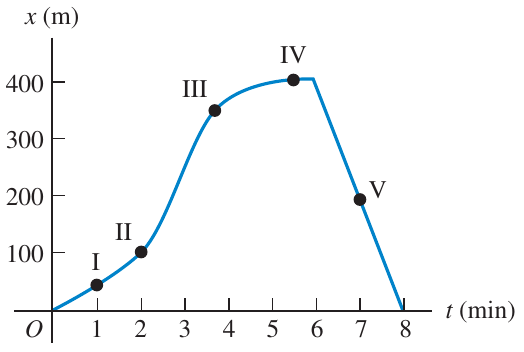
\includegraphics[width=0.4\textwidth]{figs/activ-03.png}
\end{center}
\end{multicols}
\end{exercise}
\begin{solution}
     a) IV, b) I y V, c) V, d) I, II, II IV, e) V
\end{solution}

\begin{exercise}
La siguiente tabla presenta los datos de prueba del auto más rápido fabricado. El vehículo se mueve en línea recta (el eje $x$).
\begin{center}
    \begin{tabular}{rcccc}
        \toprule
        Tiempo (\unit{s}):  & $0$ & $2.1$ & $20.0$ & $53.0$  \\
        Rapidez (\unit{km/h}): & $0$ & $96$ & $320$ & $405$ \\
        \bottomrule
    \end{tabular}
\end{center}
(a) Elabore una gráfica $v_x - t$ de la velocidad de este auto (en \unit{km/h}) en función del tiempo. ¿Su aceleración es constante?    (b) Calcule la aceleración media del auto (en \unit{m/s^2}) entre i) \num{0} y \qty{2.1}{s}; ii) \qty{2.1}{s} y \qty{20.0}{s}; iii) \qty{20.0}{s} y \qty{53}{s}. ¿Estos resultados son congruentes con el inciso a) de su gráfica?
\end{exercise}
\begin{solution}
    \begin{multicols}{2}
        a) Su aceleración no es constante, b) i) \qty{13}{m/s^2} , ii) \qty{3.48}{m/s^2}, iii) \qty{0.715}{m/s^2}, c) Si.
\begin{center}
    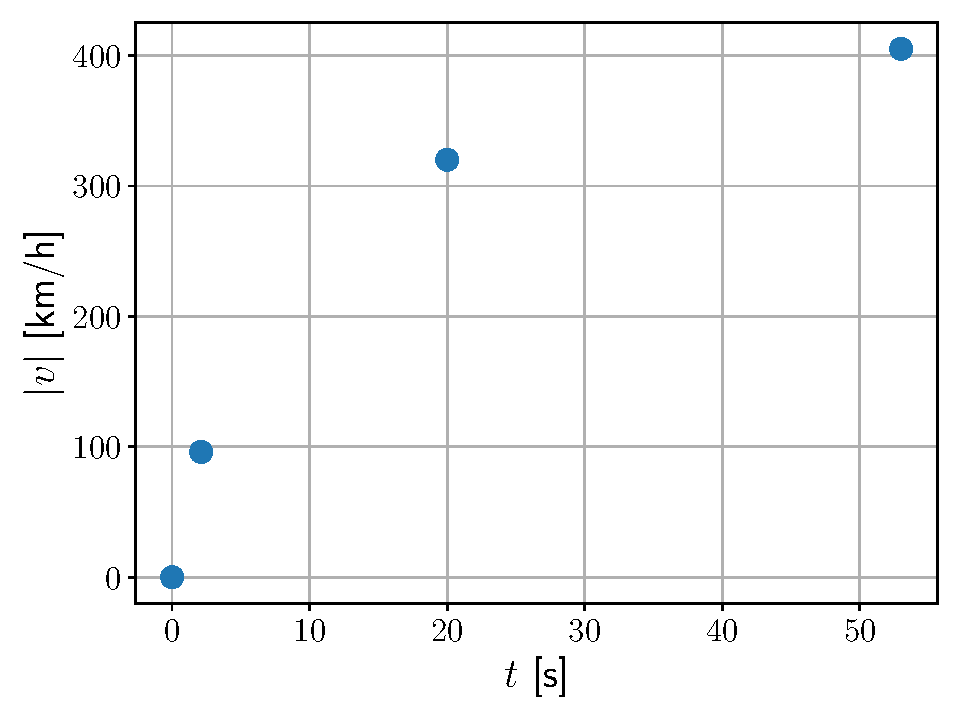
\includegraphics[width=0.4\textwidth]{figs/ac-08.pdf}
\end{center}
\end{multicols}
\end{solution}

\begin{exercise}
\begin{multicols}{2}
La figura es una gráfica de la coordenada de una araña que camina sobre el eje $x$. a) Grafique su velocidad y aceleración en función del tiempo. b) En un diagrama del eje $x$ muestre la posición, velocidad y aceleración de la araña en los cinco tiempos: $t = \qty{2.5}{s}$, $t = \qty{10}{s}$, $t = \qty{20}{s}$, $t = \qty{30}{s}$ y $t = \qty{37.5}{s}$.
\begin{center}
    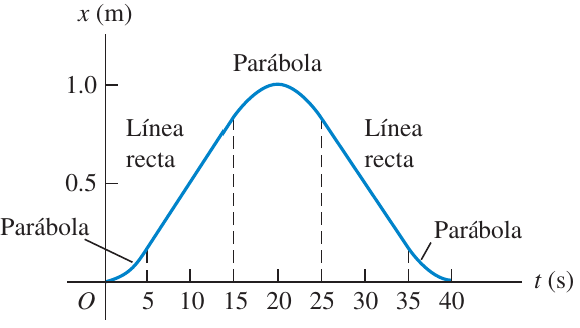
\includegraphics[width=0.5\textwidth]{figs/activ-04.png}
\end{center}
\end{multicols}
\end{exercise}
\begin{solution}
    Las flechas azules corresponden a la velocidad y las rojas a la aceleración.
\begin{center}
    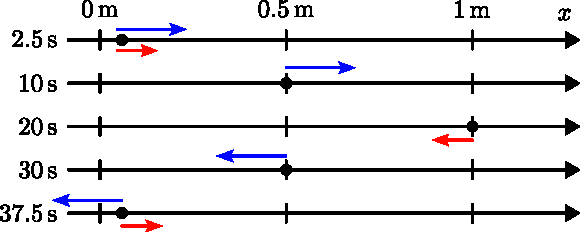
\includegraphics[width=0.5\textwidth]{figs/ac-09.pdf}
\end{center}
\end{solution}

\begin{exercise}
    \begin{wrapfigure}[5]{r}{0.3\textwidth}
\begin{center}
    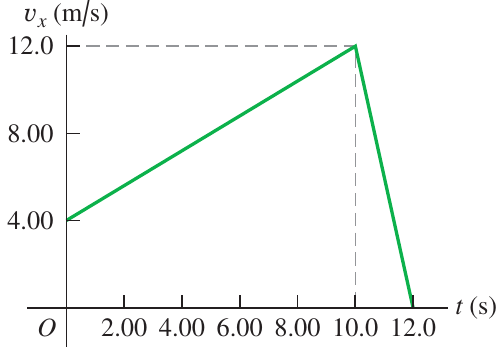
\includegraphics[width=0.3\textwidth]{figs/activ-05.png}
\end{center}
\end{wrapfigure}
    Una gacela corre en línea recta (el eje $x$). La gráfica muestra la velocidad de este animal en función del tiempo. Obtenga a) la distancia total recorrida y b) el desplazamiento de la gacela. c) Dibuje una gráfica $a_x - t$ que muestre la aceleración de esta gacela en función del tiempo durante los primeros \qty{12.0}{s}.
\end{exercise}

\begin{solution}
    a) \qty{92.0}{m} b) \qty{92.0}{m} $\bm{i}$.
\end{solution}

\begin{exercise}
    \begin{multicols}{2}
Mientras conduce, quizás usted haya notado que la velocidad de su automóvil no continúa incrementándose aun cuando mantenga su pie presionando el pedal del acelerador. Este comportamiento se debe a la resistencia del aire y a la fricción entre las partes móviles del vehículo. La figura muestra una gráfica $v_x - t$ cualitativa para un auto ordinario, cuando éste parte del reposo en el origen y viaja en línea recta (el eje $x$). Dibuje las gráficas $a_x - t$ y $x - t$ cualitativas para este automóvil.
\begin{center}
    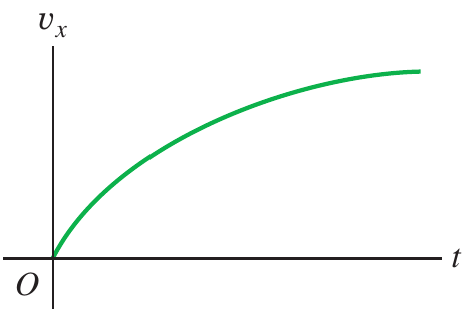
\includegraphics[width=0.35\textwidth]{figs/activ-06.png}
\end{center}
    \end{multicols}
\end{exercise}
\begin{solution}
\begin{center}
    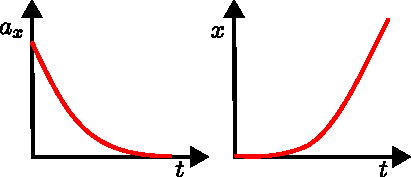
\includegraphics[width=0.5\textwidth]{figs/ac-11.pdf}
\end{center}
\end{solution}

\begin{exercise}
    \begin{multicols}{2}
        El tripulante de un globo aerostático, que sube verticalmente con velocidad constante de magnitud \qty{5.00}{m/s} (ver figura), suelta un saco de arena cuando el globo está a \qty{40.0}{m} sobre el suelo. Después de que se suelta, el saco está en caída libre. a) Calcule la posición y velocidad del saco a \qty{0.250}{s} y \qty{1.00}{s} después de soltarse. b) ¿Cuántos segundos tardará el saco en chocar con el suelo después de soltarse? c) ¿Con qué rapidez chocará? d) ¿Qué altura máxima alcanza el saco sobre el suelo? e) Dibuje las gráficas $a_y - t$, $v_y - t$ y $y - t$ para el movimiento.
\begin{center}
    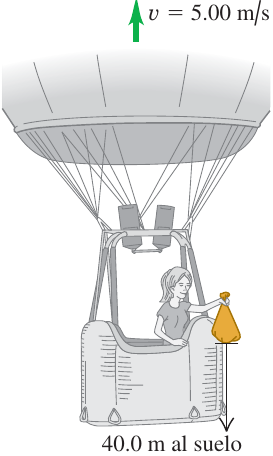
\includegraphics[width=0.2\textwidth]{figs/activ-12.png}
\end{center}
    \end{multicols}
\end{exercise}
\begin{solution}
    a) $\qty{0.250}{s} \mapsto \qty{40.9}{m}$, $\qty{1.00}{s} \mapsto \qty{40.1}{m}$, b) \qty{3.41}{s}, c) \qty{-28.4}{m/s} d) \qty{41.3}{m}, e)
\begin{center}
    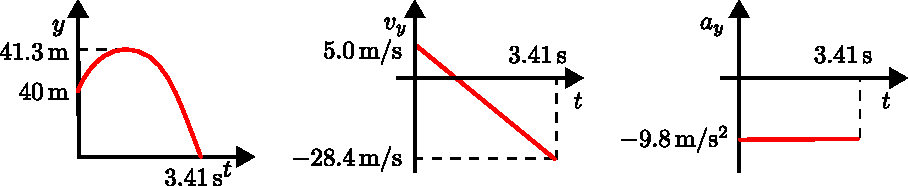
\includegraphics[width=0.7\textwidth]{figs/ac-12.pdf}
\end{center}
\end{solution}

\begin{exercise}
\begin{multicols}{2}
        Imagine que está en la azotea de un edificio, a \qty{46.0}{m} del suelo (ver figura). Una persona, que tiene una estatura de \qty{1.80}{m}, camina hacia el edificio a una rapidez constante de \qty{1.20}{m/s}. Si usted quiere dejar caer un huevo sobre su cabeza, ¿dónde deberá estar la persona cuando usted suelte el huevo? Suponga que el huevo está en caída libre.
\begin{center}
    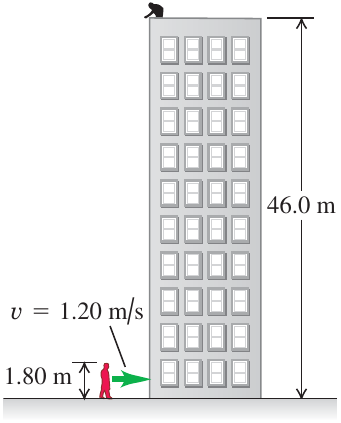
\includegraphics[width=0.25\textwidth]{figs/activ-13.png}
\end{center}
\end{multicols}
\end{exercise}
\begin{solution}
    Debe estar a \qty{10.8}{m} del edificio.
\end{solution}

\begin{exercise}
    El maquinista de un tren de pasajeros que viaja a \qty{25.0}{m/s} avista un tren de carga cuyo  vagón final está \qty{200}{m} más adelante en la misma vía. El tren de carga viaja en la misma dirección a \qty{15.0}{m/s}. El maquinista del tren de pasajeros aplica de inmediato los frenos, causando una aceleración constante de \qty{-0.100}{m/s^2}, mientras el tren de carga sigue con rapidez constante. Sea $x = 0$ el punto donde está el frente del tren de pasajeros cuando el maquinista aplica los frenos. a) ¿Atestiguarán las vacas una colisión? b) Si es así, ¿dónde ocurrirá? c) Dibuje en una sola gráfica las posiciones del frente del tren de pasajeros y de la cola del tren de carga.
\end{exercise}
\begin{solution}
    \begin{multicols}{2}
    a) Si, b) a \qty{537.5}{m} del origen de coordenadas.
\begin{center}
    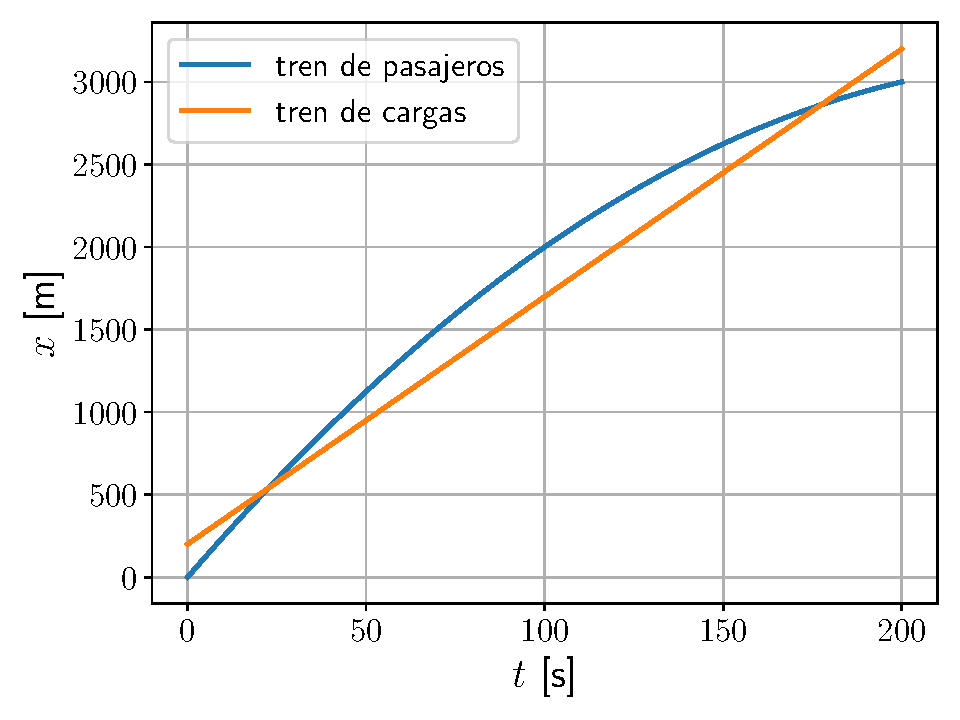
\includegraphics[width=0.45\textwidth]{figs/ac-13.pdf}
\end{center}
\end{multicols}
\end{solution}

\end{document}
